\chapter{Exploitation}
\markboth{Exploitation}{}

Adesso che sono state ottenute abbastanza informazioni sulla macchina, si può procedere con la fase di \emph{Exploitation}

\section{Strategie Automatizzate}
Il primo passo eseguito è stato quello di verificare effettivamente quali potevano essere le vulnerabilità sfruttabili consultando tutti i report ottenuti dai tool ed effettivamente le strade più promettenti sono:
\begin{enumerate}
    \item Sfruttamento della vulnerabilità di \textbf{SQL Injection};
    \item Sfruttamento della vulnerabilità di \textbf{mod\_ssl};
    \item Sfruttamento della vulnerabilità di \textbf{ProFTPD};
    \item Sfruttamento della vulnerabilità \textbf{HeartBleed};
    \item Sfruttamento di vulnerabilità di \textbf{phpMyAdmin}
\end{enumerate}

\subsection{Utilizzo di \texttt{sqlmap}}
Per tentare di sfruttare la vulnerabilità di \textbf{SQL Injection} sull'asset si è deciso di utilizzare \texttt{sqlmap}, uno strumento molto potente e in grado di automatizzare il processo di \emph{injection} sulle pagine. Per avviarlo basta eseguire il comando:
\begin{lstlisting}[language=bash]
    sqlmap -u https://10.0.2.4 -a -forms
\end{lstlisting}
dove con \texttt{-u} si specifica l'indirizzo target, con \texttt{-a} si specifica l'intenzione di voler recuperare tutto il possibile (schemi, tabelle, ecc.) e con \texttt{-forms} si specifica l'intenzione di sfruttare i \emph{form} presenti nella pagina.

Eseguendo \texttt{sqlmap} sulle varie pagine dell'asset, i risultati sono i seguenti:
\begin{figure}[h]
    \begin{subfigure}{0.5\textwidth}
        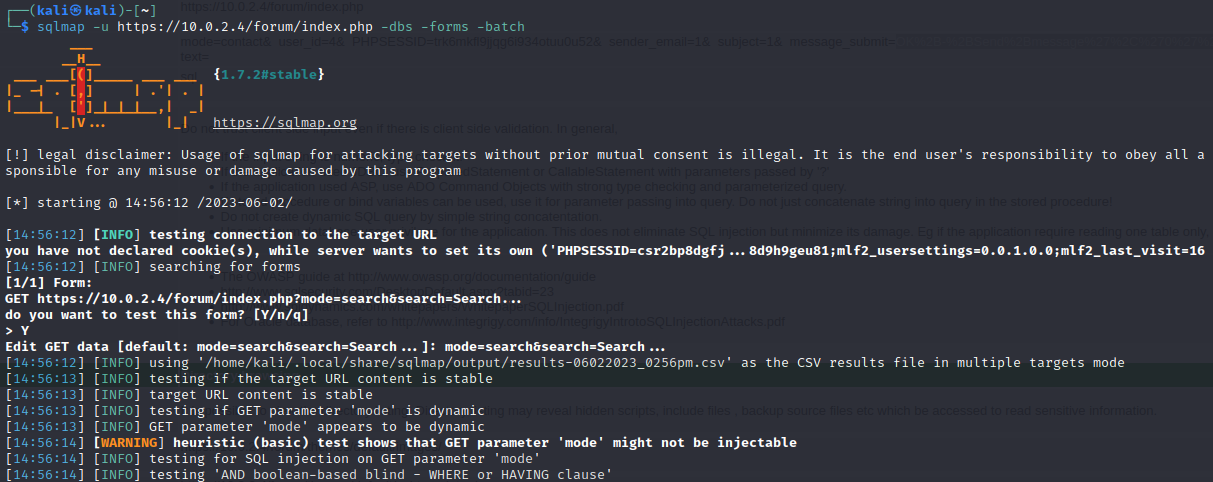
\includegraphics[width=1\textwidth]{capitoli/figure/sqlmap-forum-index-1.png}
        \caption{Prima parte del risultato parziale di \texttt{sqlmap}\\ su \emph{forum/index.php}}
        \label{fig:sqlmap-forum-index-1}
    \end{subfigure}
    \begin{subfigure}{0.5\textwidth}
        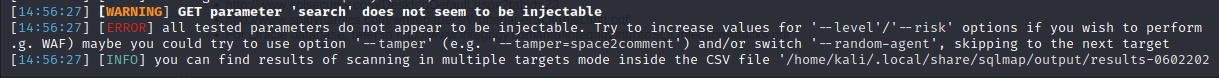
\includegraphics[width=1\textwidth]{capitoli/figure/sqlmap-forum-index-2.png}
        \caption{Seconda parte del risultato parziale di \texttt{sqlmap} su \emph{forum/index.php}}
        \label{fig:sqlmap-forum-index-2}
    \end{subfigure}
    \begin{subfigure}{0.5\textwidth}
        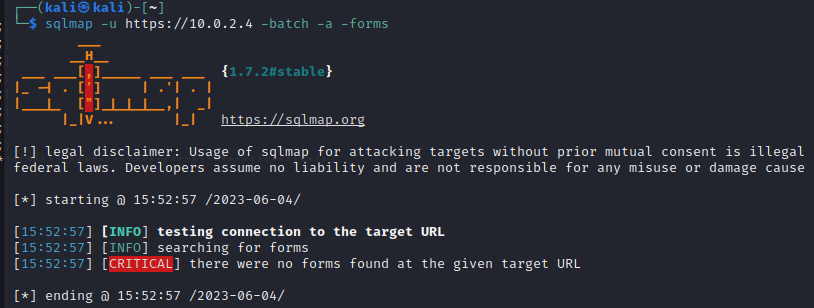
\includegraphics[width=1\textwidth]{capitoli/figure/sqlmap-index.png}
        \caption{Risultato di \texttt{sqlmap} su \emph{index.html}}
        \label{fig:sqlmap-index}
    \end{subfigure}
    \begin{subfigure}{0.5\textwidth}
        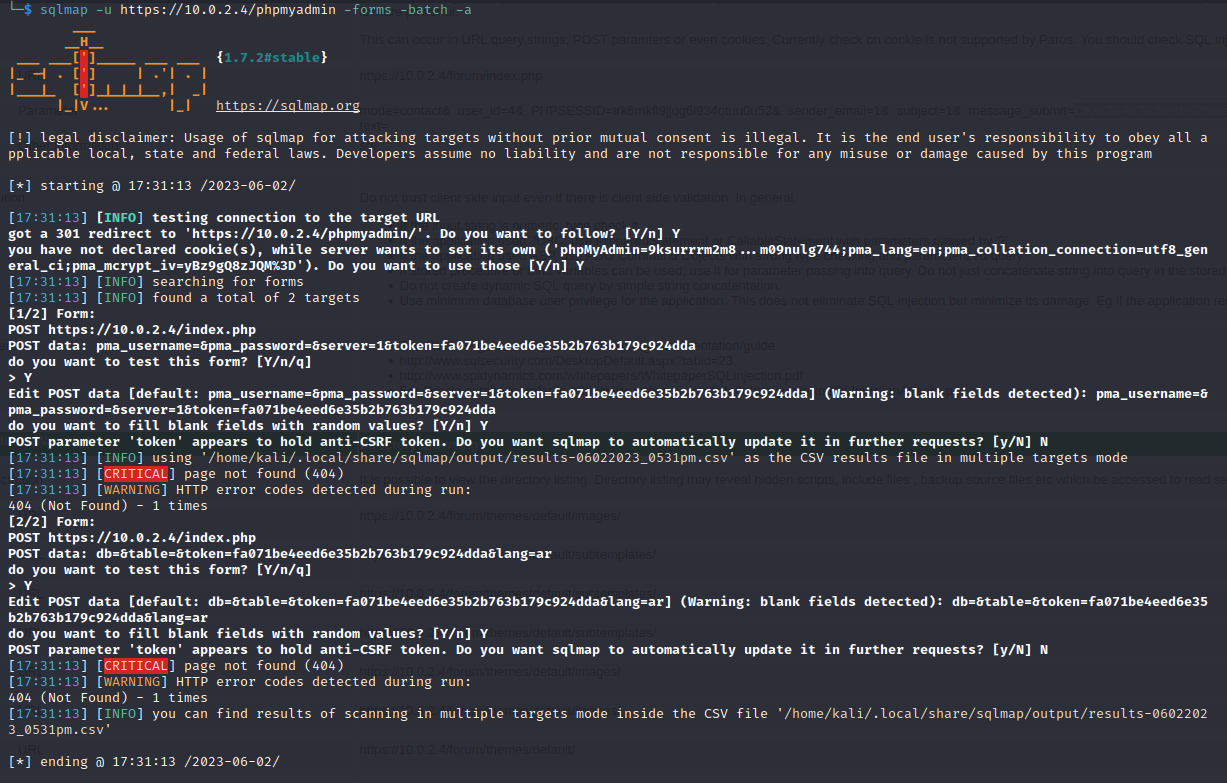
\includegraphics[width=1\textwidth]{capitoli/figure/sqlmap-phpmyadmin.png}
        \caption{Risultato di \texttt{sqlmap} su \emph{phpmyadmin}}
        \label{fig:sqlmap-phpmyadmin}
    \end{subfigure}
    \caption{Risultati ottenuti con \texttt{sqlmap}}
    \label{fig:sqlmap}
\end{figure}

Come si può notare dalle varie esecuzioni di \texttt{sqlmap} si può stabilire che purtroppo lo sfruttamento della \textbf{SQL Injection} non è praticabile e non permette di ottenere ulteriori informazioni. A questo punto, ciò che si può supporre è che il rilevamento effettuato da \texttt{paros} e da \emph{Nessus} non è altro che un falso positivo.

In vista dei risultati ottenuti, quindi, si può scartare questa strategia e procedere con le successive.

\subsection{Utilizzo della suite \emph{Metasploit}}
Il passo successivo è quello di cercare di sfruttare le altre vulnerabilità rilevate riguardo \textbf{mod\_ssl, ProFTPD, HeartBleed} e \textbf{phpMyAdmin}. Utilizzando la suite \emph{Metasploit}, quello che si può fare è cercare degli \emph{exploit} in grado di sfruttare una delle vulnerabilità rilevate dai tool utilizzati per la scansione. Per eseguire la ricerca viene quindi lanciata la console di \emph{Metasploit} con il comando \texttt{msfconsole} e successivamente viene utilizzato il comando \texttt{search}.\\
La prima ricerca effettuata riguarda \textbf{mod\_ssl} e, a quanto rivelato dal report, una versione deprecata di questo strumento potrebbe permettere addirittura l'esecuzione di codice arbitrario da remoto. Tuttavia, effettuando la ricerca non viene trovato nulla a riguardo, come mostrato di seguito:
\begin{figure}[h]
    \centering
    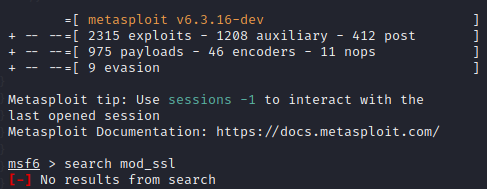
\includegraphics[width=0.5\textwidth]{capitoli/figure/metasploit-mod_ssl.png}
    \caption{Risultato ricerca di \textbf{mod\_ssl}}
    \label{fig:metasploit-modssl}
\end{figure}

Anche effettuando una ricerca sul sito del \emph{MITRE} si scopre che, nonostante questa possibilità, non sono forniti exploit a riguardo.\\
Allora quello che si può fare è continuare la ricerca con \textbf{ProFTPD} e, questa volta, si ottengono dei risultati come mostrato di seguito:
\begin{figure}[h]
    \centering
    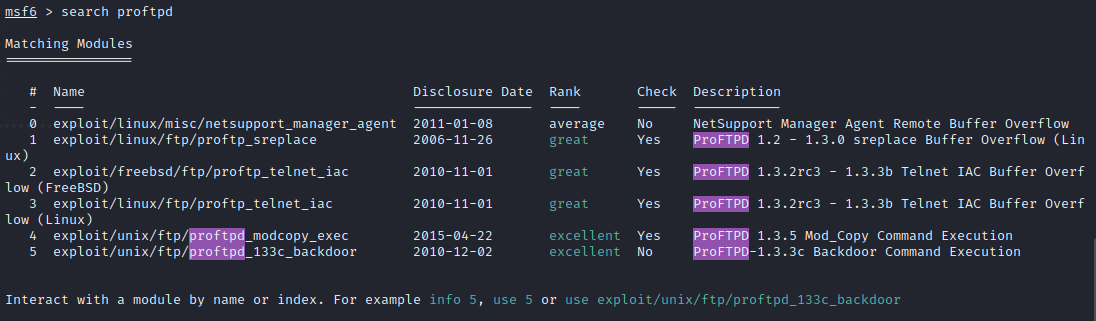
\includegraphics[width=0.6\textwidth]{capitoli/figure/metasploit-proftpd.png}
    \caption{Risultato ricerca di \textbf{ProFTPD}}
    \label{fig:metasploit-proftpd}
\end{figure}

Tenendo presente che la versione di \textbf{ProFTPD} installata è \textbf{1.3.4a}, si nota che solo un exploit potrebbe essere utilizzabile in quanto gli altri sono efficaci solo contro versioni precedenti a quella installata. L'exploit in questione è \textbf{modcopy\_exec} che permette la copia di qualunque file accessibile con i permessi dell'utente che esegue il servizio \textbf{ProFTPD} e anche esecuzione di codice tramite \emph{PHP} \cite{proftpd-mod-copy}.

Selezionando questo exploit e come payload una reverse shell con \emph{netcat} (con le opportune configurazioni),  il risultato è che non si ha successo poichè probabilmente non si hanno i permessi di scrittura sulla cartella target, come mostrato di seugito:
\begin{figure}[h]
    \centering
    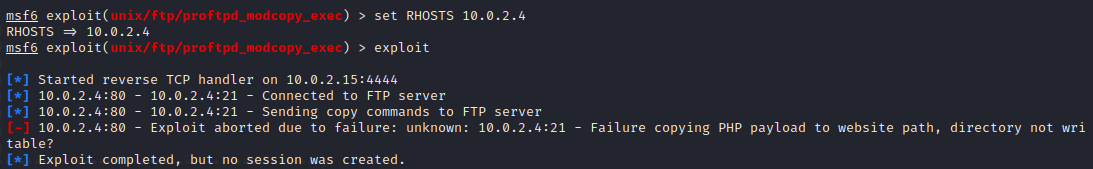
\includegraphics[width=0.5\textwidth]{capitoli/figure/metasploit-proftpd-attack.png}
    \caption{Risultato attacco di \textbf{ProFTPD}}
    \label{fig:metasploit-proftpd-attack}
\end{figure}

Lo stesso risultato è ottenuto anche con tutti gli altri payload, sia di tipo reverse che di tipo bind, rendendo anche questa strada non utilizzabile.\\
Rimossa anche quest'altra strada, un ulteriore tentativo è quello di sfruttare \textbf{HeartBleed}. Come fatto in precedenza, viene effettuata la ricerca di exploit a riguardo e il risultato è il seguente:
\begin{figure}[h]
    \centering
    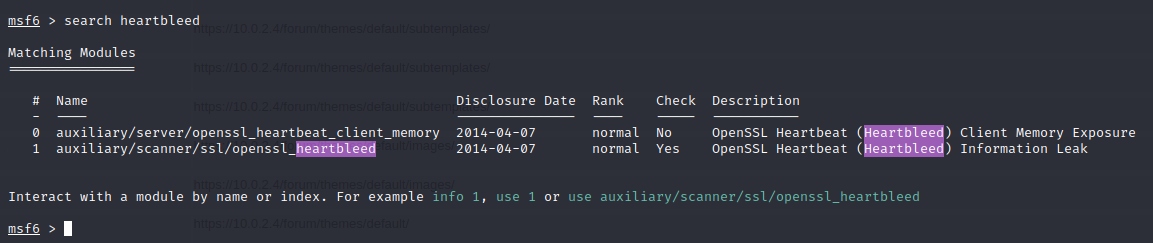
\includegraphics[width=0.7\textwidth]{capitoli/figure/metasploit-heartbleed-list.png}
    \caption{Risultato ricerca di \textbf{HeartBleed}}
    \label{fig:metasploit-heartbleed}
\end{figure}

Non è stato trovato un exploit a riguardo ma un modulo ausiliario, il quale non permette di ottenere una \emph{shell} (quindi il controllo della macchina), ma permette l'ottenimento di altre informazioni che possono tornare molto utili. Se ad esempio si riuscisse a sfruttare questa vulnerabilità, si potrebbero ottenere persino password e chiavi private salvate sul server. Utilizzando lo scanner, tuttavia, il risultato è che ancora una volta non si riesce ad ottenere nulla, come mostrato di seguito:
\begin{figure}[h]
    \centering
    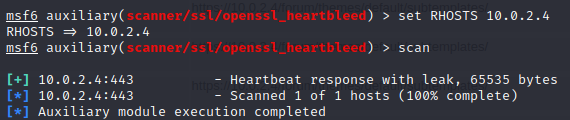
\includegraphics[width=0.6\textwidth]{capitoli/figure/metasploit-heartbleed-scan.png}
    \caption{Risultato attacco con \textbf{HeartBleed}}
    \label{fig:metasploit-heartbleed-attack}
\end{figure}

Infatti l'esecuzione del modulo termina senza ottenere nulla, confermando però la presenza della vulnerabilità \textbf{HeartBleed}.\\
A questo punto non resta che sperare in qualche vulnerabilità di \textbf{phpMyAdmin} (visto che era stata rilevato un falso positivo magari c'è altro) e, effettuando una ricerca, si ottengono i seguenti risultati:
\begin{figure}[h]
    \centering
    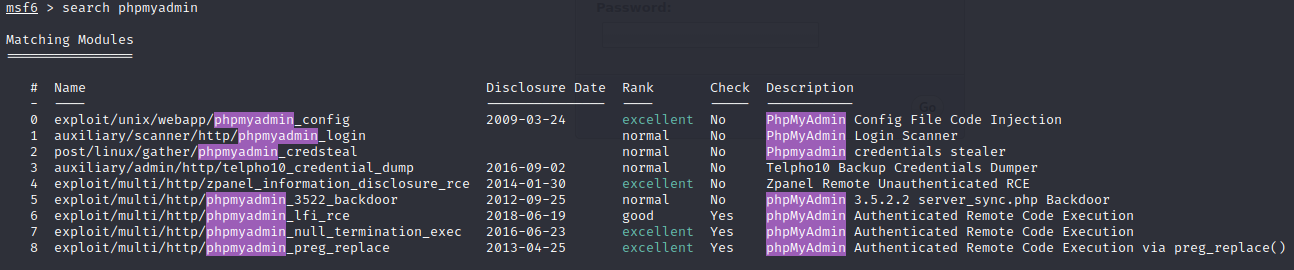
\includegraphics[width=0.7\textwidth]{capitoli/figure/metasploit-phpmyadmin.png}
    \caption{Risultato ricerca di \textbf{phpMyAdmin}}
    \label{fig:metasploit-phpmyadmin}
\end{figure}

Escludendo i moduli \emph{post} (Utilizzabili dopo aver eseguito l'exploitation con successo) e \emph{auxiliary}, gli unici \emph{exploit} interessanti sono gli ultimi 3. Sfortunatamente, dopo l'esecuzione di tutti i payload di tutti e 3 gli exploit, non è stato possibile eseguire l'exploiting della macchina \emph{10.0.2.4}, come mostrato parzialmente di seguito:
\begin{figure}[h]
    \centering
    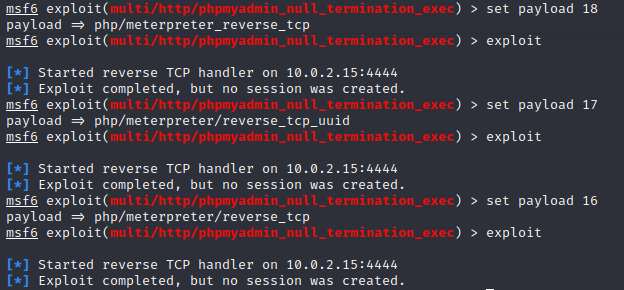
\includegraphics[width=0.7\textwidth]{capitoli/figure/metasploit-phpmyadmin-attack.png}
    \caption{Risultato parziale dell'attacco a \textbf{phpMyAdmin}}
    \label{fig:metasploit-phpmyadmin-attack}
\end{figure}

Purtroppo, dopo quest'ultimo fallimento, non sembrano esserci altre vie percorribili basandosi sulle informazioni acquisite in precedenza.

\subsection{Utilizzo della GUI \emph{Armitage}}
Un ultimo tentativo che è possibile realizzare è quello di utlizzare \emph{Armitage}, una GUI per la suite \emph{Metasploit}. Il motivo è per utilizzare una funzione offerta chiamata \textbf{Hail Mary}, che si occupa di effettuare il bruteforce di tutti gli exploit e payload compatibili su una macchina target nella speranza di instaurare almeno una \emph{sessione}. Per utilizzare la funzione precedentemente citata, bisogna effettuare di nuovo le fasi target discovery ed enumeration all'interno di \emph{Armitage} e, una volta finite, basta utilizzare l'opzione \emph{find attacks} per filtrare gli exploit che sono compatibili con la macchina target. Il risultato ottenuto fino a questo momento è il seguente:
\begin{figure}[h]
    \centering
    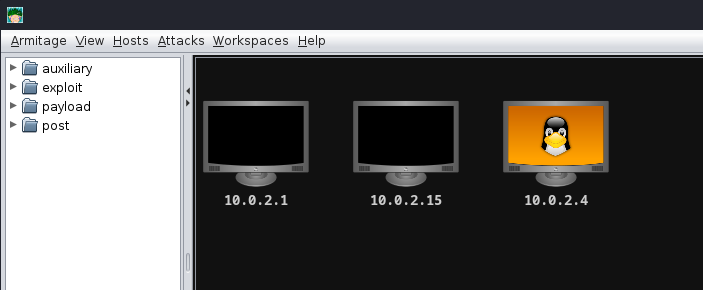
\includegraphics[width=0.7\textwidth]{capitoli/figure/armitage.png}
    \caption{Output di \emph{Armitage} dopo le scansioni}
    \label{fig:armitage}
\end{figure}

A questo punto è possibile lanciare la funzione \emph{Hail Mary} e, dopo aver atteso che tutti gli exploit siano stati lanciati, si può osservare che anche con questa strategia \emph{estrema} non è stato possibile avere accesso alla macchina. Un report con gli exploit lanciati da questa funzione è consultabile nella cartella \emph{Report} con il nome \textbf{armitage-hailmary.log}.

\subsection{Fallimento delle strategie automatizzate}
Nonostante i report fossero promettenti inizialmente, visto che sono state trovate trovate vulnerabilità interessanti, l'utilizzo di strumenti automatici per l'exploitation non ha mostrato i risultati sperati e si è rivelato un completo fallimento. Una possibile ragione per cui questo è accaduto può essere il fatto che l'asset da attaccare in realtà è una macchina che non è stata pensata per un \emph{Penetration Testing} ma bensì per una \emph{sfida CTF}. Questo significa, quindi, che la macchina non è stata realizzata utilizzando servizi vulnerabili (sarebbe stata facilitata la risoluzione della \emph{sfida CTF}) ma utilizzando servizi "aggiornati" (ovviamente in riferimento alle versioni dell'anno di rilascio) che non presentano vulnerabilità tali da fornire accesso completo o parziale alla macchina e navigazione libera del file system della macchina ma che permettono ugualmente di effettuare la \emph{CTF}. In base a questa osservazione non ci sono quindi altri modi per avere accesso alla macchina se non quello di risolvere la sfida interrogando manualmente la macchina ed estrapolando nuove informazioni fornite dai servizi offerti.

\section{Strategie manuali}
La decisione presa, a questo punto, è quella di procedere con l'analisi manuale dell'asset.
\subsection{Visita del server web}
La prima interazione eseguita è semplicemente quella di interrogare l'asset in maniera legittima sulla porta 80. L'output che si può osservare è il seguente:
\begin{figure}[h]
    \centering
    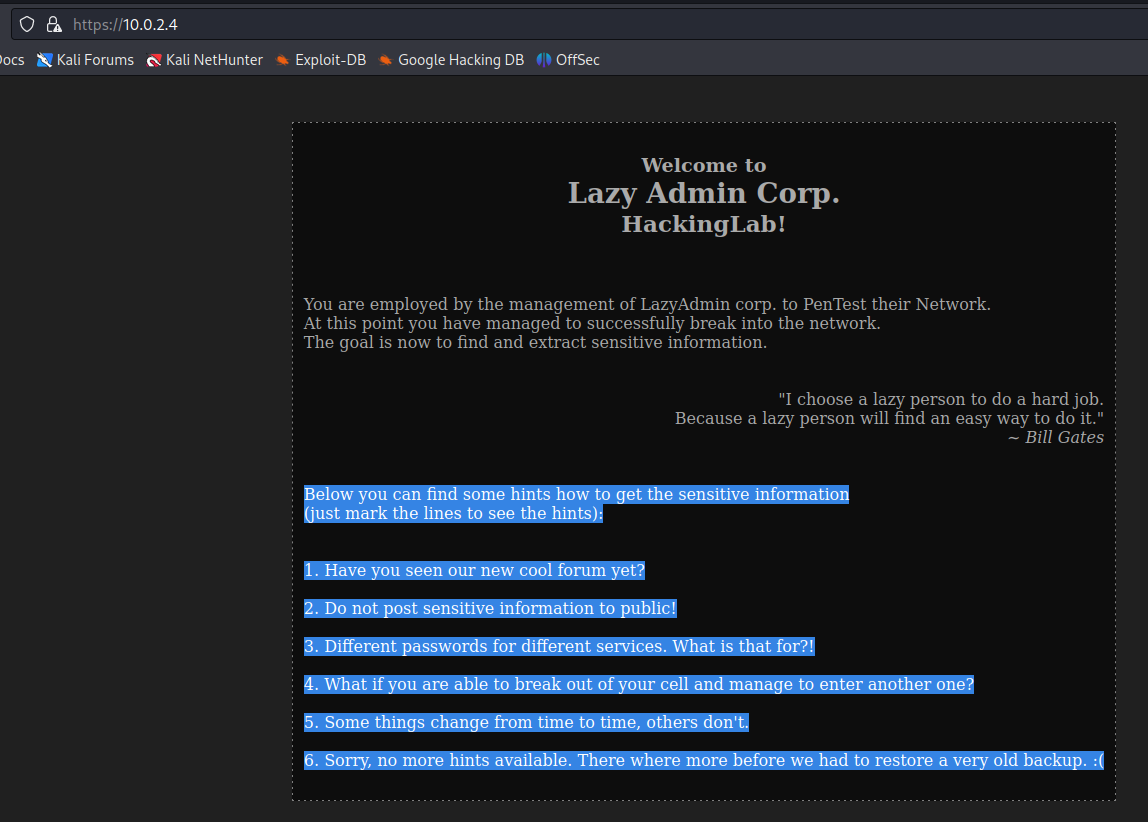
\includegraphics[width=0.5\textwidth]{capitoli/figure/web-index.png}
    \caption{Welcome page dell'asset}
    \label{fig:web-index}
\end{figure}

Evidenziando il testo (come indicato nel suggerimento) si possono ricavare informazioni molto utili:
\begin{itemize}
    \item Viene indicata la presenza di un \textbf{forum}, che già era noto dall'output di \texttt{dirb} e \texttt{nikto};
    \item Viene specificato che non dovrebbero essere \emph{postate} informazioni sensibili in pubblico, quasi come se qualcuno avesse postato delle credenziali (verosimilmente) sul forum;
    \item La presenza di un \textbf{backup} molto vecchio che è stato ripristinato;
\end{itemize}

Non sembrano esserci ulteriori informazioni utili sulla pagina, quindi si può procedere.

\subsection{Accesso al servizio \emph{FTP}}
Prima di continuare con la visita delle pagine web, dalle scansioni precedenti è stato rilevato che il servizio \textbf{ProFTPD} ammette login \emph{anonimi}, per cui vale la pena di tentare una connessione e capire se ci sono file utili a cui si hanno accesso. Eseguendo una connessione anonima, il risultato è il seguente:
\begin{figure}[h]
    \centering
    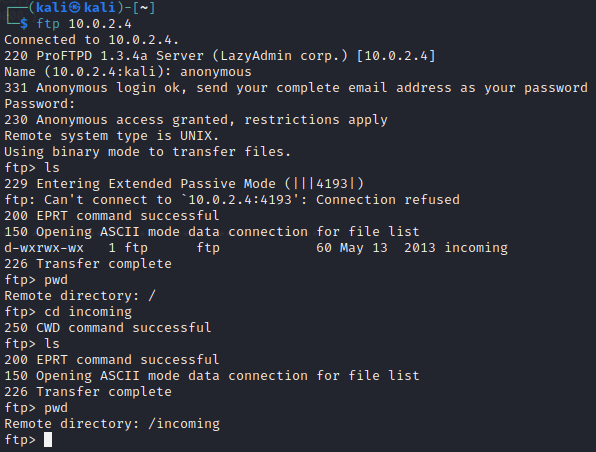
\includegraphics[width=0.5\textwidth]{capitoli/figure/ftp-anon.png}
    \caption{Login anonimo sul servizio \emph{FTP}}
    \label{fig:ftp-anon}
\end{figure}

Quello che si nota è che purtroppo si ha accesso solo ad una cartella di nome \textbf{incoming} che è vuota. Molto probabilmente questo è dovuto al fatto che con il login anonimo non si hanno i permessi per visualizzare il contenuto della suddetta cartella. Quindi al momento non è possibile accedere a nessun file presente sull'asset, però, il nome della cartella ricorda il nome di una \emph{casella di posta} (in italiano \emph{In arrivo}) e questa informazione è coerente anche con la presenza della pagina \textbf{webmail} rilevata da \texttt{nikto}. Ad ogni modo, si può tornare con la consultazione delle pagine web.

\subsection{Analisi della pagina forum}
In base alle informazioni prese dalla \emph{welcome page} dell'asset, il prossimo passo è la visita della pagina \emph{forum}. La pagina si presenta come mostrato di seguito:
\begin{figure}[h]
    \centering
    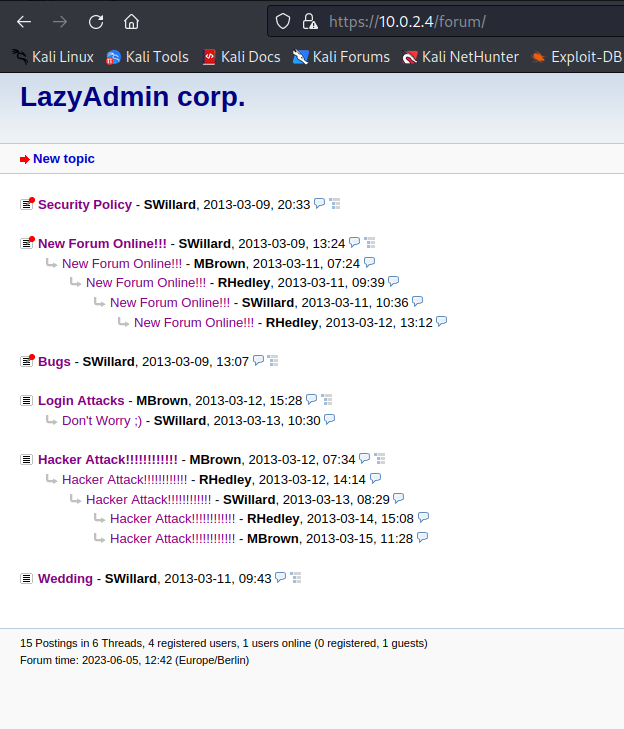
\includegraphics[width=0.4\textwidth]{capitoli/figure/forum.png}
    \caption{Pagina web del \emph{forum}}
    \label{fig:forum}
\end{figure}

Visitando le varie discussioni presenti, salta all'occhio una discussione con il nome \textbf{Login Attacks}, il cui contenuto parziale è mostrato di seguito:
\begin{figure}[h]
    \centering
    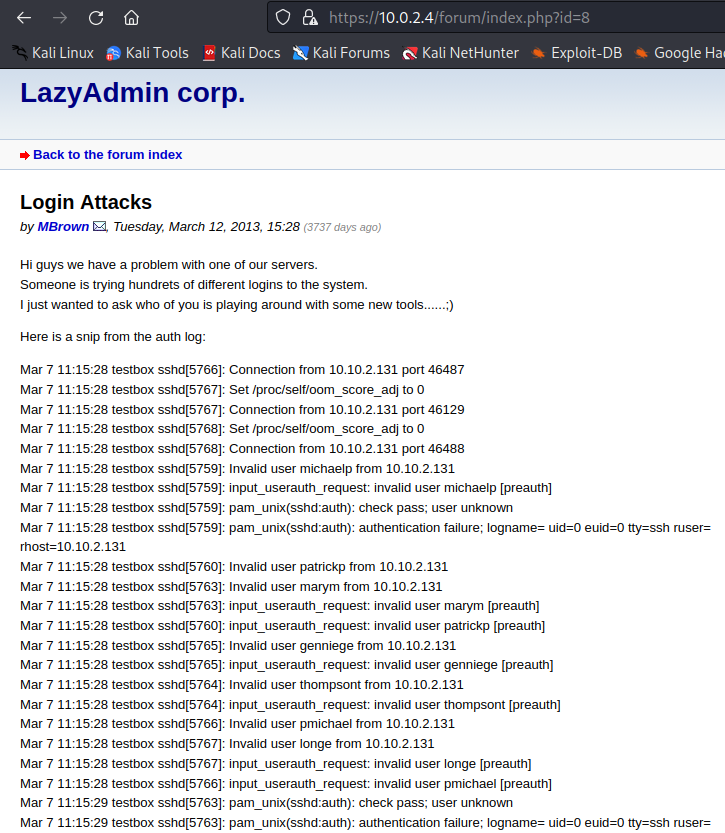
\includegraphics[width=0.4\textwidth]{capitoli/figure/forum-ssh-log.png}
    \caption{Contenuto parziale della discussione \textbf{Login Attacks}}
    \label{fig:forum-ssh-log}
\end{figure}

Leggendo la discussione, si nota che il contenuto riguarda un log di accessi falliti tramite \emph{SSH}. Copiando l'intero contenuto su un file di testo, è stato utilizzato il comando \texttt{grep} per estrarre i nomi utente utilizzati nell'attacco in maniera più agevole e veloce. I nomi utente rilevati sono i seguenti:
\begin{figure}[h]
    \centering
    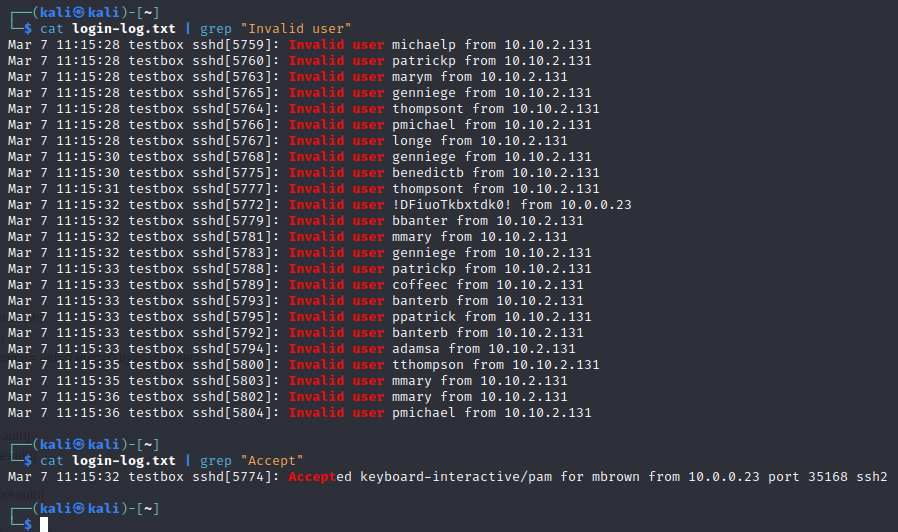
\includegraphics[width=0.4\textwidth]{capitoli/figure/ssh-log-grep.png}
    \caption{Nomi utente estratti con \texttt{grep}}
    \label{fig:ssh-log-grep}
\end{figure}

Dai risultati si possono notare 2 aspetti particolari:
\begin{itemize}
    \item C'è un unico login riuscito con il nome utente \textbf{mbrown}
    \item È presente il nome utente \textbf{!DFiuoTkbxtdk0!} che non sembra avere esattamente l'aspetto di un nome utente ma, piuttosto, sembra essere una \emph{password}.
\end{itemize}

\subsection{Compromissione di un utente del forum}
Notando che il nome dell'utente che ha postato la discussione è proprio \textbf{MBrown}, presente anche nei log trovati, è lecito supporre che l'utente \textbf{mbrown} presente nell'attacco sia lo stesso del forum. Per questo motivo, per la stranezza di uno dei nomi utente (evidenziato in precedenza) e per la tendenza delle persone ad usare la stessa password per servizi diversi, vale la pena tentare un attacco a dizionario sul login del forum con tutte le combinazioni dei nomi utente. Dopo alcuni tentativi falliti, una combinazione funzionante è stata:
\begin{itemize}
    \item \textbf{Nome Utente}: mbrown
    \item \textbf{Password}: !DFiuoTkbxtdk0!
\end{itemize}
Questo ha confermato i sospetti sulla stranezza del nome utente, e il login con le credenziali ci ha dato accesso alla pagina personale dell'utente \textbf{mbrown}, che ha il seguente aspetto:
\begin{figure}[h]
    \centering
    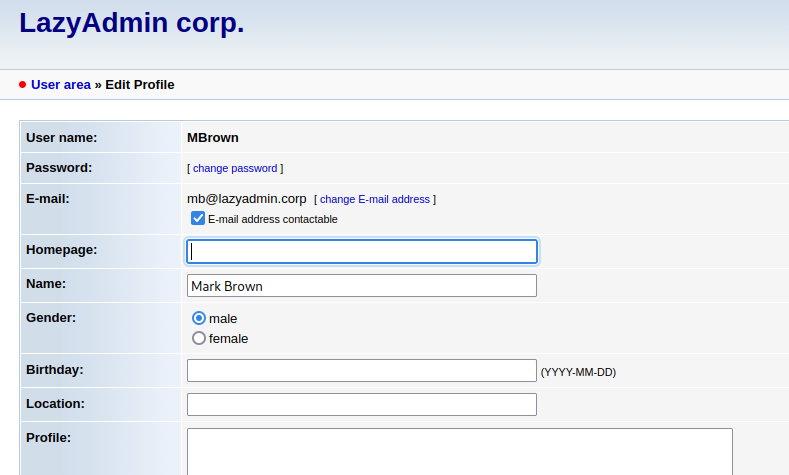
\includegraphics[width=0.4\textwidth]{capitoli/figure/forum-accesso.png}
    \caption{Pagina personale dell'utente \textbf{mbrown}}
    \label{fig:forum-accesso}
\end{figure}

L'unica informazione che sembra essere utile all'interno della pagina è la mail dell'utente compromesso, che è \textbf{mb@lazyadmin.corp}. A questo punto, ricordandoci anche della presenza di una pagina \emph{webmail}, vale la pena tentare l'accesso sulla \emph{webmail} specificando la mail appena trovata e la password appena utilizzata, sfruttando ancora la tendenza delle persone ad utilizzare la stessa password per servizi diversi.

Inaspettatamente, il tentativo ha successo e viene mostrata la pagina seguente:
\begin{figure}[h]
    \centering
    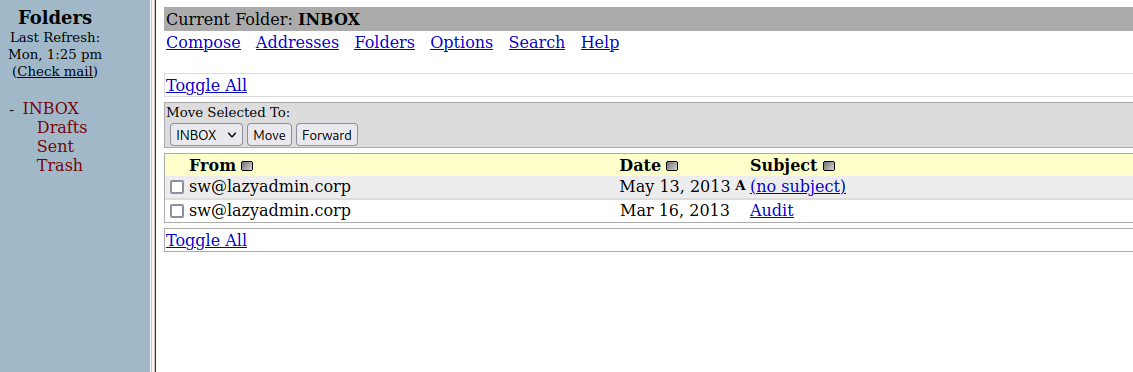
\includegraphics[width=0.5\textwidth]{capitoli/figure/mail-accesso.png}
    \caption{Pagina \emph{webmail} dell'utente \textbf{mbrown}}
    \label{fig:mail-accesso}
\end{figure}

Sono presenti due mail e il contenuto di una delle due è il seguente:
\begin{figure}[h]
    \centering
    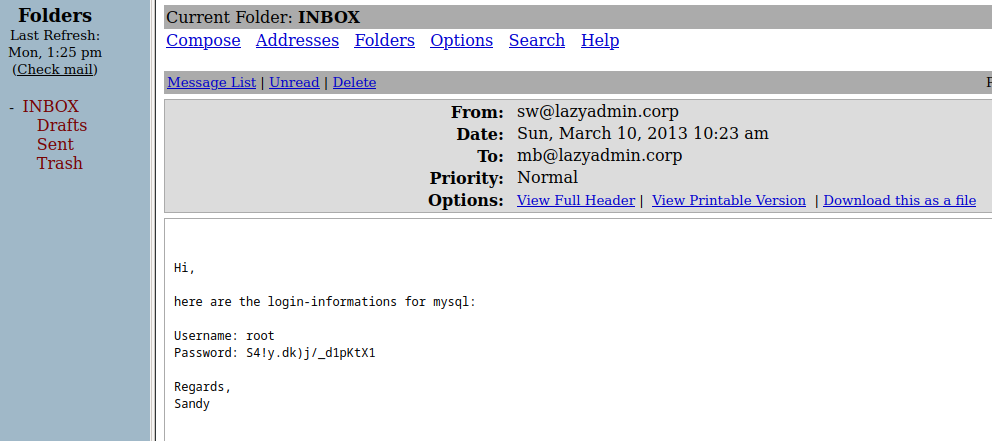
\includegraphics[width=0.5\textwidth]{capitoli/figure/mail-password.png}
    \caption{Una delle mail dell'utente \textbf{mbrown}}
    \label{fig:mail-password}
\end{figure}

È stata comunicata la password dell'utente \textbf{root} del servizio \textbf{phpMyAdmin}.

\subsection{Compromissione di \textbf{phpMyAdmin}}
Ovviamente, andando sulla pagina \emph{phpmyadmin} e immettendo le credenziali ottenute dalla mail, il risultato è che si riesce ad accedere come utente \textbf{root} e viene visualizzata la pagina mostrata di seguito:
\begin{figure}[h]
    \centering
    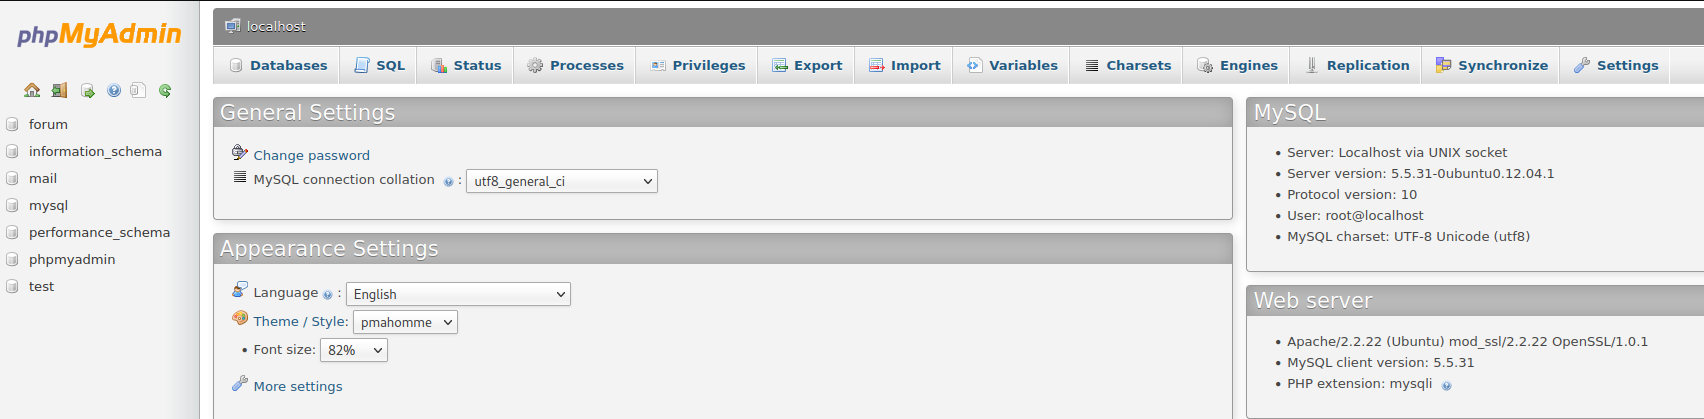
\includegraphics[width=0.5\textwidth]{capitoli/figure/phpmyadmin.png}
    \caption{Pagina dell'utente \textbf{root} su \emph{phpmyadmin}}
    \label{fig:phpmyadmin}
\end{figure}

Esplorando un po' i database presenti, sono di particolare interesse i database \textbf{forum} e \textbf{mail} dove tra tutte le tabelle presenti ci sono delle tabelle una chiamata \emph{ mlf2\_userdata} e l'altra \emph{mailbox}. Aprendo queste tabelle si possono recuperare gli hash delle password di alcuni degli utenti.

\subsection{Cracking degli hash ottenuti}
Questi hash recuperati sono stati salvati in un file e dati in pasto ad un tool di \emph{Offline Password cracking} chiamato \texttt{john} che, dopo un po' di tentativi con wordlist diverse, non è riuscito ad ottenere le corrispondenti password. Dal momento che l'utilizzo di altri strumenti con le stesse \emph{wordlist} si suppone che diano lo stesso risultato, si è tentato di sfruttare risorse sul web nella speranza che qualcuno abbia effettuato il cracking degli hash ottenuti. La ricerca è iniziata su \emph{crackstation.com} dove sfortunatamente non è stato trovato nulla e, successivamente, con una semplice ricerca su \emph{google} degli hash, è stato trovato il sito \emph{md5.gromweb.com} dove è stato possibile reperire 3 password. Il risultato ottenuto è mostrato di seguito:
\begin{figure}[h]
    \centering
    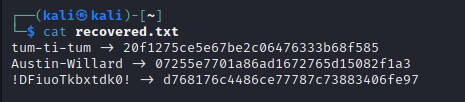
\includegraphics[width=0.7\textwidth]{capitoli/figure/hash-recovered.png}
    \caption{Le tre password recuperate}
    \label{fig:hash-recovered}
\end{figure}

Le password sono rispettivamente di \textbf{Richard Hedley} e \textbf{Sandy Willard}, due utenti che sono iscritti sul forum con i nomi \textbf{RHedley} e \textbf{SWillard}.

\subsection{Tentativo di accesso}
Ora che sono state recuperate le password di tre utenti, quello che si può fare è tentare di accedere al sistema con uno di questi, tuttavia ancora non si conoscono i nomi utenti del sistema ma solo quelli del forum. Ricordando per un attimo il log trovato sul forum, si può notare che un tentativo di accesso riuscito è stato realizzato con il nome utente \textbf{mbrown}, l'utente di cui è stato violato l'account del forum. Un tentativo che si può fare è utilizzare questo nome utente per provare ad accedere al sistema tramite \emph{SSH} o \emph{FTP} utilizzando la password che è stata scoperta. Tuttavia il risultato è mostrato nella Figura \ref{fig:ssh-ftp-incorrect}
\begin{figure}[h]
    \centering
    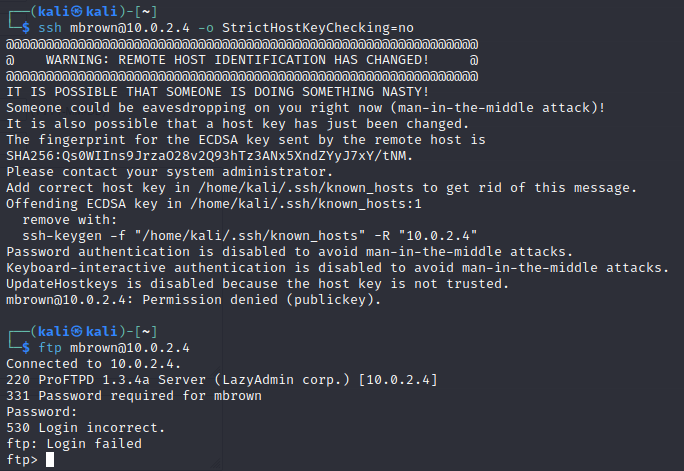
\includegraphics[width=0.6\textwidth]{capitoli/figure/ssh-ftp-incorrect.png}
    \caption{Tentativi di login con l'utente \textbf{mbrown}}
    \label{fig:ssh-ftp-incorrect}
\end{figure}

Per quanto concerne \emph{SSH} essendo che la macchina \textbf{Kali} non è un host riconosciuto, l'autenticazione tramite password è disabilitata e viene richiesto un file di autenticazione (una chiave con cui autenticare la chiave pubblica), quindi non è possibile al momento utilizzare \emph{SSH} (verosimilmente anche con gli altri utenti).\\
Invece, per quanto riguarda \emph{FTP}, a quanto sembra la password non è la stessa che è stata utilizzata in precedenza quindi non si può effettuare il login con l'utente \textbf{mbrown}.

\subsection{Accesso al servizio FTP come nuovo utente}
Essendo che l'utente \textbf{Mark Brown} ha come nome utente sul forum \textbf{MBrown} e come nome utente di sistema \textbf{mbrown}, molto probabilmente questo schema è mantenuto anche dagli altri utenti del sistema. Seguendo questo presupposto, viene effettuato un tentativo con l'utente \textbf{Richard Hedley} e, con un po' di fortuna, il risultato è il seguente:
\begin{figure}[h]
    \centering
    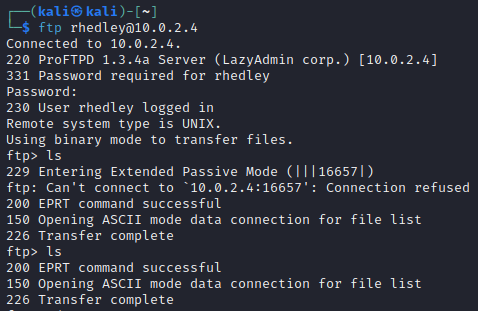
\includegraphics[width=0.5\textwidth]{capitoli/figure/ftp-rhedley.png}
    \caption{Accesso \emph{FTP} con l'utente \textbf{rhedley}}
    \label{fig:ftp-rhedley}
\end{figure}

È stato eseguito il login con successo e, a questo punto, quello che si può fare è esplorare un po' i file accessibili dall'utente. Quello che si può notare è che l'utente utilizzato ha accesso alla cartella dell'utente \textbf{mbrown} e andando nella cartella \textbf{.ssh} (dove \emph{OpenSSH} salva i file relativi alle chiavi) si trova un file \textbf{downloadkey} al quale l'utente può accedere, come mostrato di seguito:
\begin{figure}[h]
    \begin{subfigure}{0.6\textwidth}
        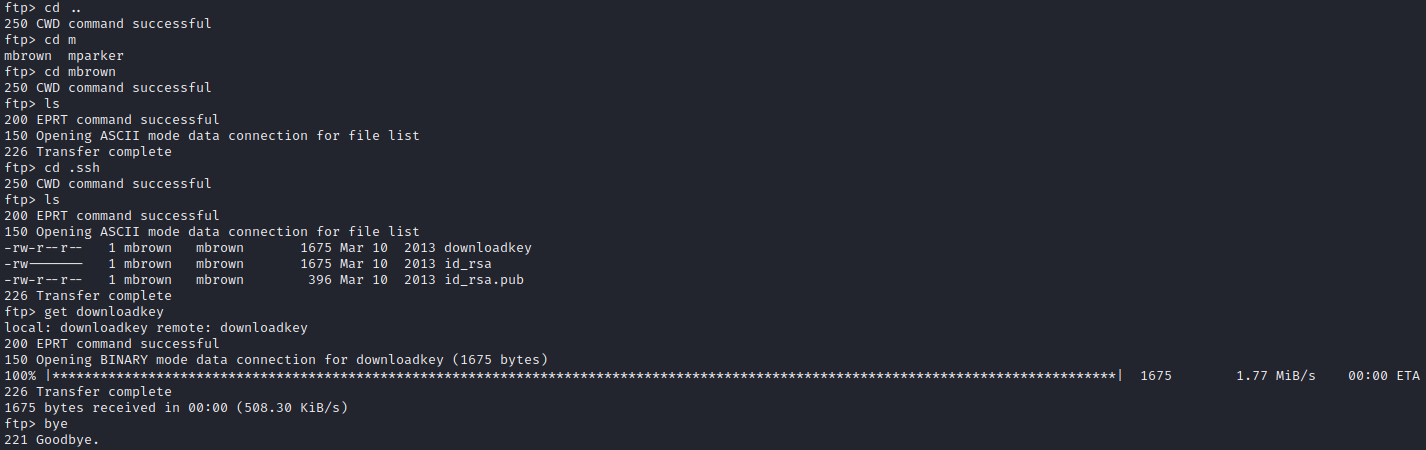
\includegraphics[width=1\textwidth]{capitoli/figure/ftp-rhedley-private-key.png}
        \caption{Download della chiave di \textbf{mbrown}}
        \label{fig:ftp-rhedley-private}
    \end{subfigure}
    \begin{subfigure}{0.4\textwidth}
        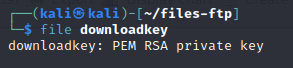
\includegraphics[width=1\textwidth]{capitoli/figure/file-downloadkey.png}
        \caption{Verifica della tipologia di chiave di \textbf{mbrown}}
        \label{fig:file-downloadkey}
    \end{subfigure}
    \caption{Ottenimento della chiave privata di \textbf{mbrown}}
    \label{fig:mbrown-private-key}
\end{figure}

Una volta ottenuto il file \textbf{downloadkey}, utilizzando il comando \texttt{file} è stato possibile accertarsi che il file sia effettivamente una \textbf{chiave privata}.

\subsection{Ottenimento di una shell}
Dal momento che grazie all'utente \textbf{rhedley} è stato possibile recuperare la chiave privata dell'utente \textbf{mbrown}, adesso è possibile effettuare l'accesso all'asset tramite \emph{SSH} utilizzando il seguente comando:
\begin{lstlisting}[language=bash]
    ssh -i downloadkey mbrown@10.0.2.4 -o StrictHostKeyChecking=no
\end{lstlisting}

È stato necessario aggiungere anche il parametro \texttt{StrictHostKeyChecking=no} poichè, dal momento che ad ogni riavvio l'asset rigenera la propria chiave \emph{SSH}, \emph{OpenSSH} solleva un warning e chiude la connessione in via preventiva per evitare attacchi \textbf{Man-In-The-Middle} (visto che la chiave pubblica precedentemente salvata è cambiata) e, per evitare la chiusura, si aggiunge il parametro per ignorare quest'allerta.\\
In seguito all'esecuzione del comando, il risultato è il seguente:
\begin{figure}[h]
    \centering
    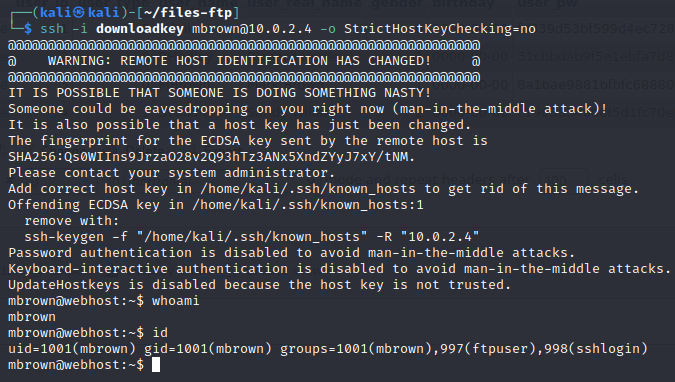
\includegraphics[width=0.5\textwidth]{capitoli/figure/ssh-mbrown.png}
    \caption{Ottenimento della shell come utente \textbf{mbrown}}
    \label{fig:ssh-mbrown}
\end{figure}

Adesso che è stata ottenuta una shell sull'asset, la fase di \emph{Exploitation} può dirsi conclusa con successo.